\usetikzlibrary{positioning,shapes.callouts}

\begin{frame}{Chrome architecture}
    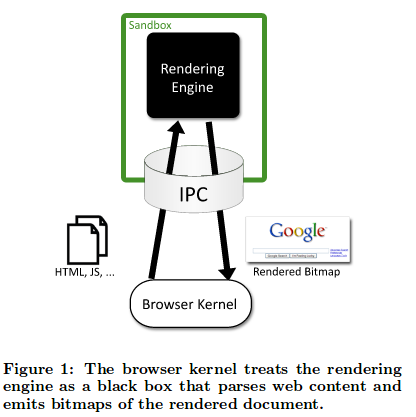
\includegraphics[height=0.8\textheight]{../sandbox/chrome-arch}
\end{frame}

\begin{frame}{talking to the sandbox}
    \begin{itemize}
    \item browser kernel sends commands to sandbox
    \item sandbox sends commands to browser kernel
    \item idea: commands only allow necessary things
    \end{itemize}
\end{frame}

\begin{frame}{original Chrome sandbox interface}
    \begin{itemize}
        \item sandbox to browser ``kernel''
            \begin{itemize}
                \item show this image on screen
                \begin{itemize}
                    \item (using shared memory for speed)
                \end{itemize}
            \item \myemph<2-3>{make request\tikzmark{request} for this URL}
            \item \myemph<4>{download\tikzmark{download} files to local FS}
            \item \myemph<5>{upload\tikzmark{upload} user requested files}
            \end{itemize}
        \item browser ``kernel'' to sandbox
            \begin{itemize}
                \item send user input
            \end{itemize}
    \end{itemize}
    \begin{tikzpicture}[overlay,remember picture]
        \coordinate (middle) at ([yshift=-1cm]current page.center);
        \begin{visibleenv}<2>
            \node[my callout=request,anchor=center,align=center]  at (middle) {
                needs filtering --- at least no \texttt{file:} (local file) URLs
            };
        \end{visibleenv}
        \begin{visibleenv}<3>
            \node[my callout=request,anchor=center,align=center] at (middle) {
                can still read any website! \\
                still sends normal cookies!
            };
        \end{visibleenv}
        \begin{visibleenv}<4>
            \node[my callout=download,anchor=center,align=center] at (middle) {
                files go to download directory only \\
                can't choose arbitrary filenames
            };
        \end{visibleenv}
        \begin{visibleenv}<5>
            \node[my callout=upload,anchor=center,align=center] at ([yshift=-1cm]middle) {
                browser kernel displays file choser \\
                only permits files selected by user
            };
        \end{visibleenv}
    \end{tikzpicture}
\end{frame}

